\documentclass[11pt, a4paper]{article}
\usepackage{pdfpages}
\usepackage{parallel}
\usepackage[T2A]{fontenc}
\usepackage{ucs}
\usepackage[utf8x]{inputenc}
\usepackage[polish,english,russian]{babel}
\usepackage{hyperref}
\usepackage{rotating}
\usepackage[inner=2cm,top=1.8cm,outer=2cm,bottom=2.3cm,nohead]{geometry}
\usepackage{listings}
\usepackage{graphicx}
\usepackage{wrapfig}
\usepackage{longtable}
\usepackage{indentfirst}
\usepackage{array}
\usepackage{tikzsymbols}
\usepackage{soul}
\usepackage[ruled,vlined]{algorithm2e}
%\counterwithout{figure}{section} 

\usepackage{url}
\makeatletter
\g@addto@macro{\UrlBreaks}{\UrlOrds}
\makeatother

\newcolumntype{P}[1]{>{\raggedright\arraybackslash}p{#1}}
\frenchspacing
\usepackage{fixltx2e} %text sub- and superscripts
\usepackage{icomma} % коскі ў матэматычным рэжыме
\PreloadUnicodePage{4}

\newcommand{\longpage}{\enlargethispage{\baselineskip}}
\newcommand{\shortpage}{\enlargethispage{-\baselineskip}}

\def\switchlang#1{\expandafter\csname switchlang#1\endcsname}
\def\switchlangbe{
\let\saverefname=\refname%
\def\refname{Літаратура}%
\def\figurename{Іл.}%
}
\def\switchlangen{
\let\saverefname=\refname%
\def\refname{References}%
\def\figurename{Fig.}%
}
\def\switchlangru{
\let\saverefname=\refname%
\let\savefigurename=\figurename%
\def\refname{Литература}%
\def\figurename{Рис.}%
}

\hyphenation{admi-ni-stra-tive}
\hyphenation{ex-pe-ri-ence}
\hyphenation{fle-xi-bi-li-ty}
\hyphenation{Py-thon}
\hyphenation{ma-the-ma-ti-cal}
\hyphenation{re-ported}
\hyphenation{imp-le-menta-tions}
\hyphenation{pro-vides}
\hyphenation{en-gi-neering}
\hyphenation{com-pa-ti-bi-li-ty}
\hyphenation{im-pos-sible}
\hyphenation{desk-top}
\hyphenation{elec-tro-nic}
\hyphenation{com-pa-ny}
\hyphenation{de-ve-lop-ment}
\hyphenation{de-ve-loping}
\hyphenation{de-ve-lop}
\hyphenation{da-ta-ba-se}
\hyphenation{plat-forms}
\hyphenation{or-ga-ni-za-tion}
\hyphenation{pro-gramming}
\hyphenation{in-stru-ments}
\hyphenation{Li-nux}
\hyphenation{sour-ce}
\hyphenation{en-vi-ron-ment}
\hyphenation{Te-le-pathy}
\hyphenation{Li-nux-ov-ka}
\hyphenation{Open-BSD}
\hyphenation{Free-BSD}
\hyphenation{men-ti-on-ed}
\hyphenation{app-li-ca-tion}

\def\progref!#1!{\texttt{#1}}
\renewcommand{\arraystretch}{2} %Іначай формулы ў матрыцы зліпаюцца з лініямі
\usepackage{array}

\def\interview #1 (#2), #3, #4, #5\par{

\section[#1, #3, #4]{#1 -- #3, #4}
\def\qname{LVEE}
\def\aname{#1}
\def\q ##1\par{{\noindent \bf \qname: ##1 }\par}
\def\a{{\noindent \bf \aname: } \def\qname{L}\def\aname{#2}}
}

\def\interview* #1 (#2), #3, #4, #5\par{

\section*{#1\\{\small\rm #3, #4. #5}}
\ifx\ParallelWhichBox\undefined%
    \addcontentsline{toc}{section}{#1, #3, #4}%
\else%
\ifnum\ParallelWhichBox=0%
    \addcontentsline{toc}{section}{#1, #3, #4}%
\fi\fi%

\def\qname{LVEE}
\def\aname{#1}
\def\q ##1\par{{\noindent \bf \qname: ##1 }\par}
\def\a{{\noindent \bf \aname: } \def\qname{L}\def\aname{#2}}
}

\newcommand{\interviewfooter}[1]{
\vskip 1em
\noindent \textit{#1}
}

\switchlang{ru}
\begin{document}

\title{2001 "--- Macally QBALL trackball}
\date{}
\maketitle
\selectlanguage{russian}
Трекбол QBALL был выпущен Тайваньской компанией Jiaxin Technology "--- владельцем торговой марки Macally, под которой выпускалась известная линейка периферии для компьютеров Mac.

Для компьютеров PC была выпущена аналогичная модель с незапоминающимся названием PCGB, которая продавалась под брендом Pcally, и не отличалась от Macally QBALL ничем кроме названия \cite{trackballfan}.

\begin{figure}[h]
    \centering
    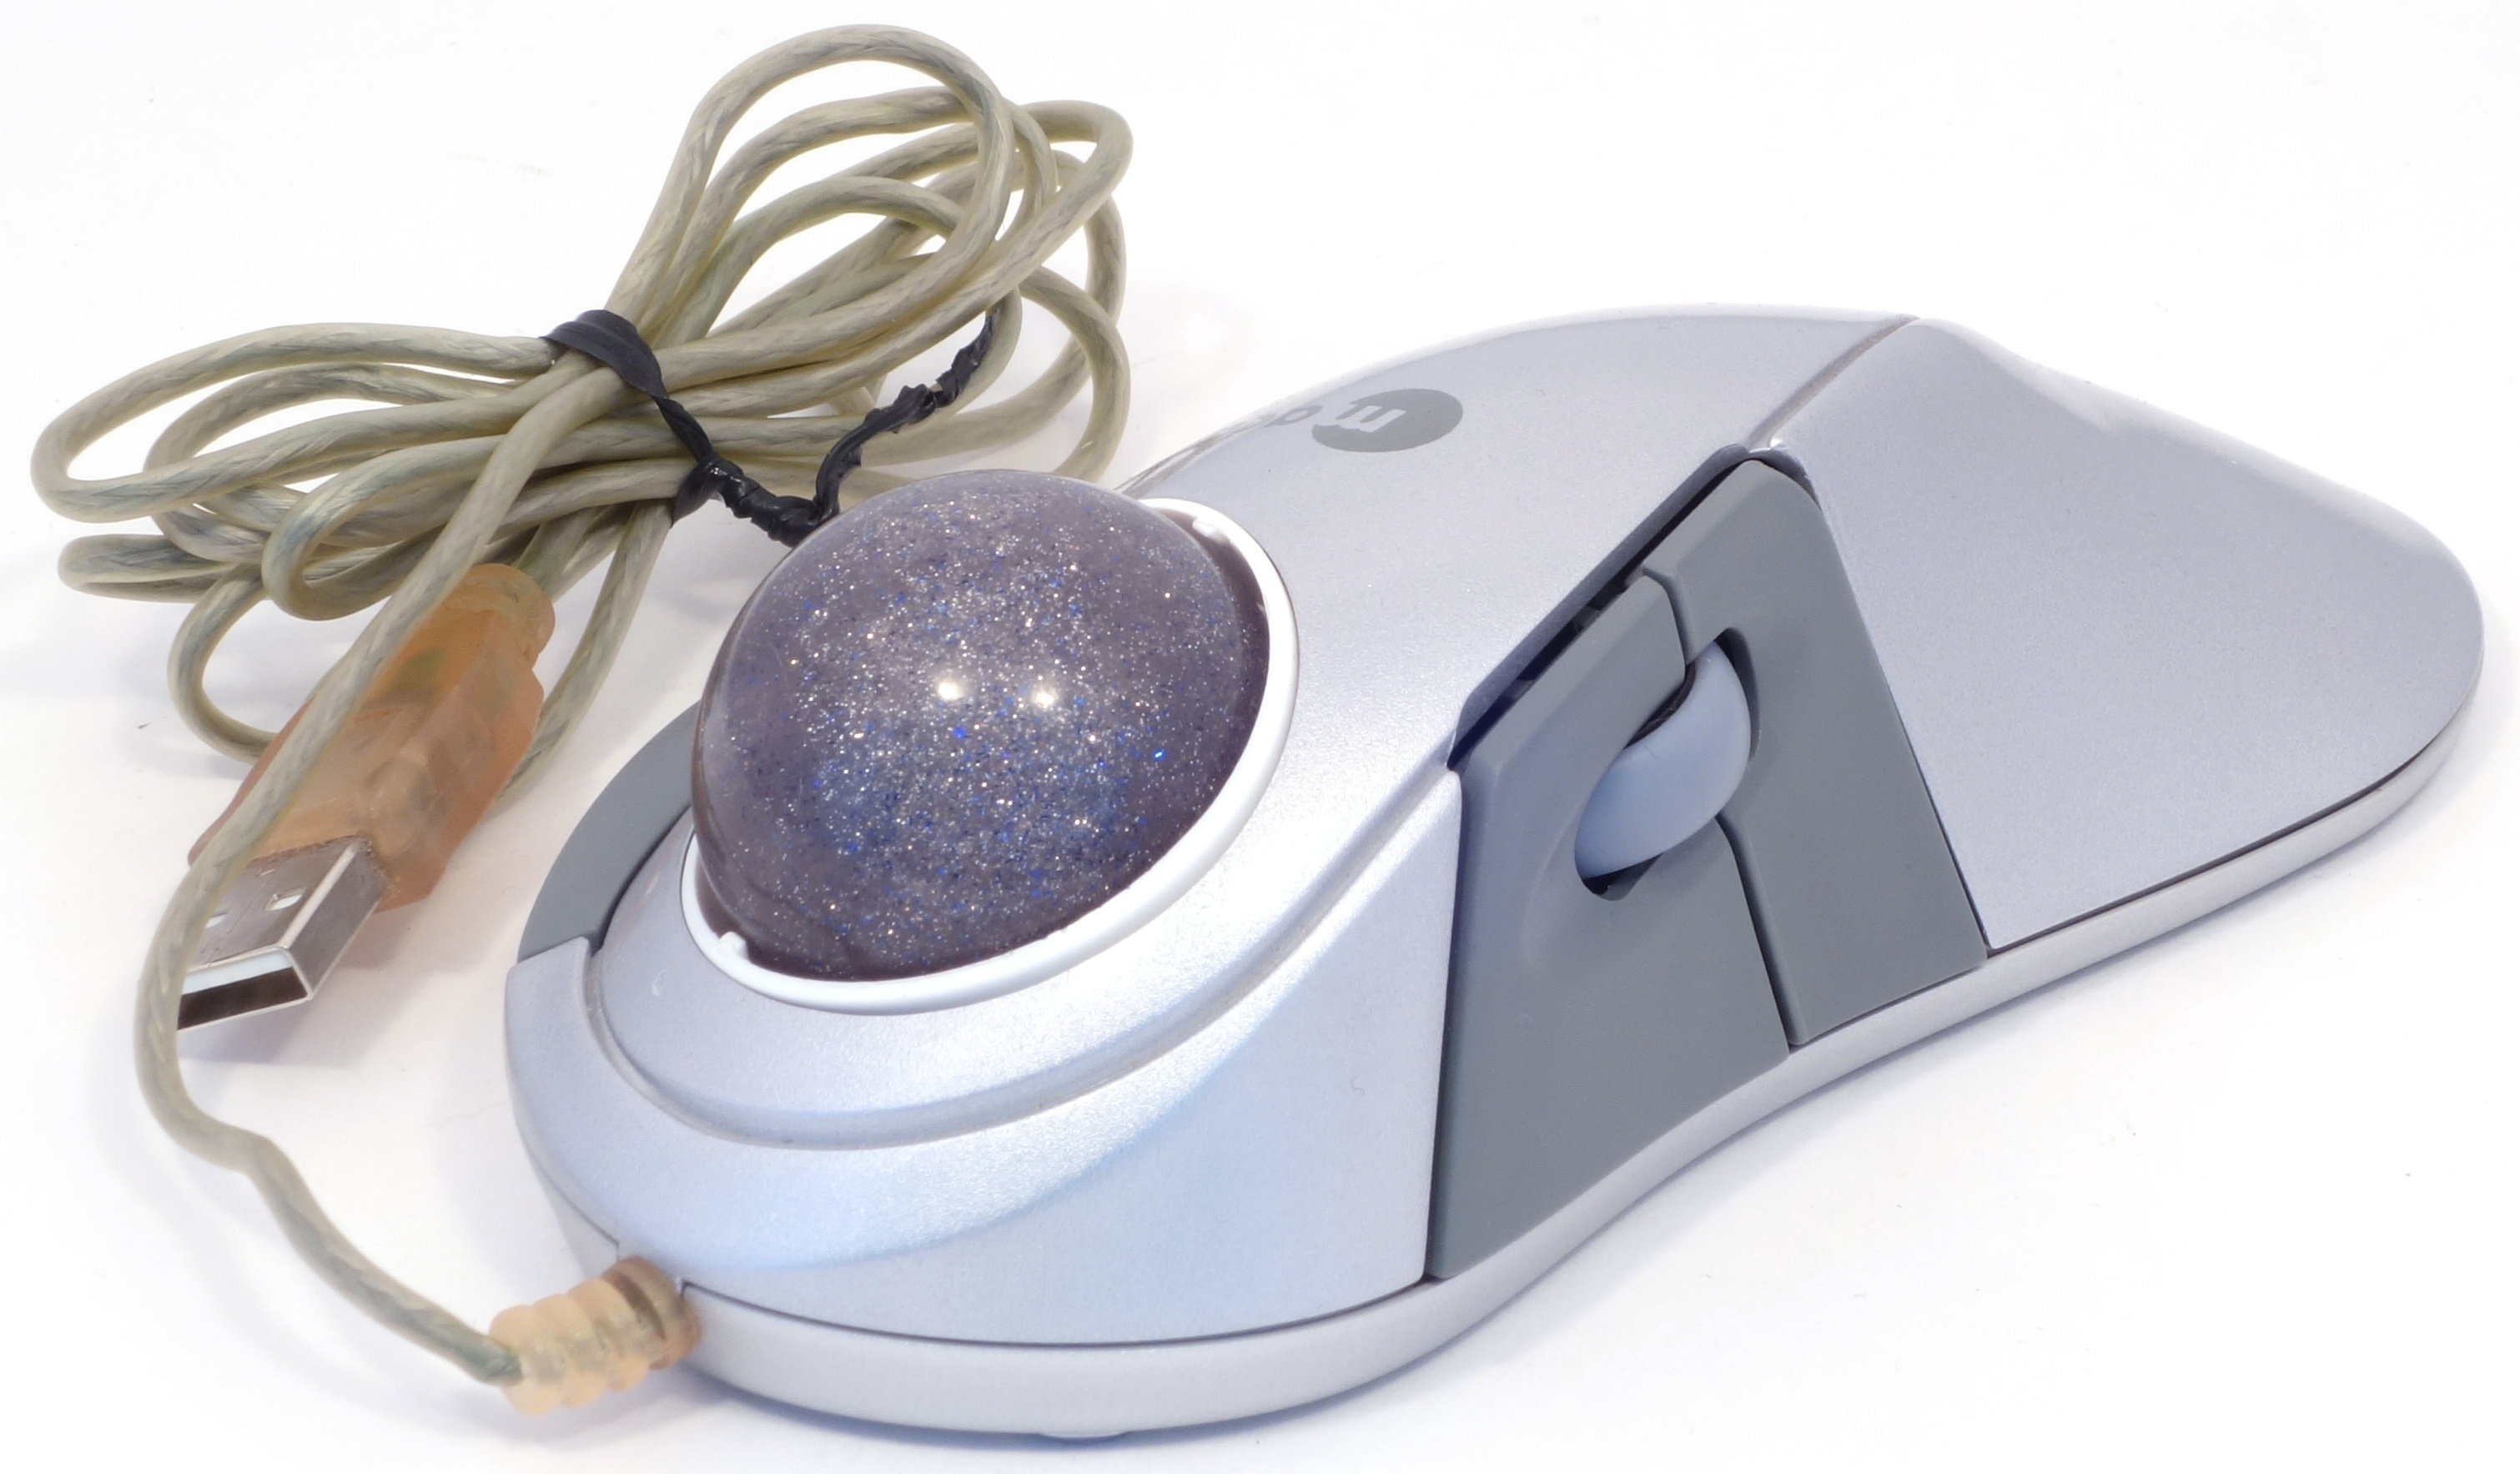
\includegraphics[scale=0.5]{2001_macally_qball/pic_30.jpg}
    \caption{Macally QBALL}
    \label{fig:MacallyQBALLPic}
\end{figure}

Особенностью трекбола является полупрозрачный шар с мелкими блестящими вкраплениями, так называнный <<Glitter Ball>> \cite{site}. В состоянии покоя шар слегка подсвечивается красным светодиодом, а в момент вращения яркость подсветки усиливается \cite{review}, облегчая оптическому датчику регистрацию движения содержащихся в шаре вкраплений.

\begin{figure}[h]
    \centering
    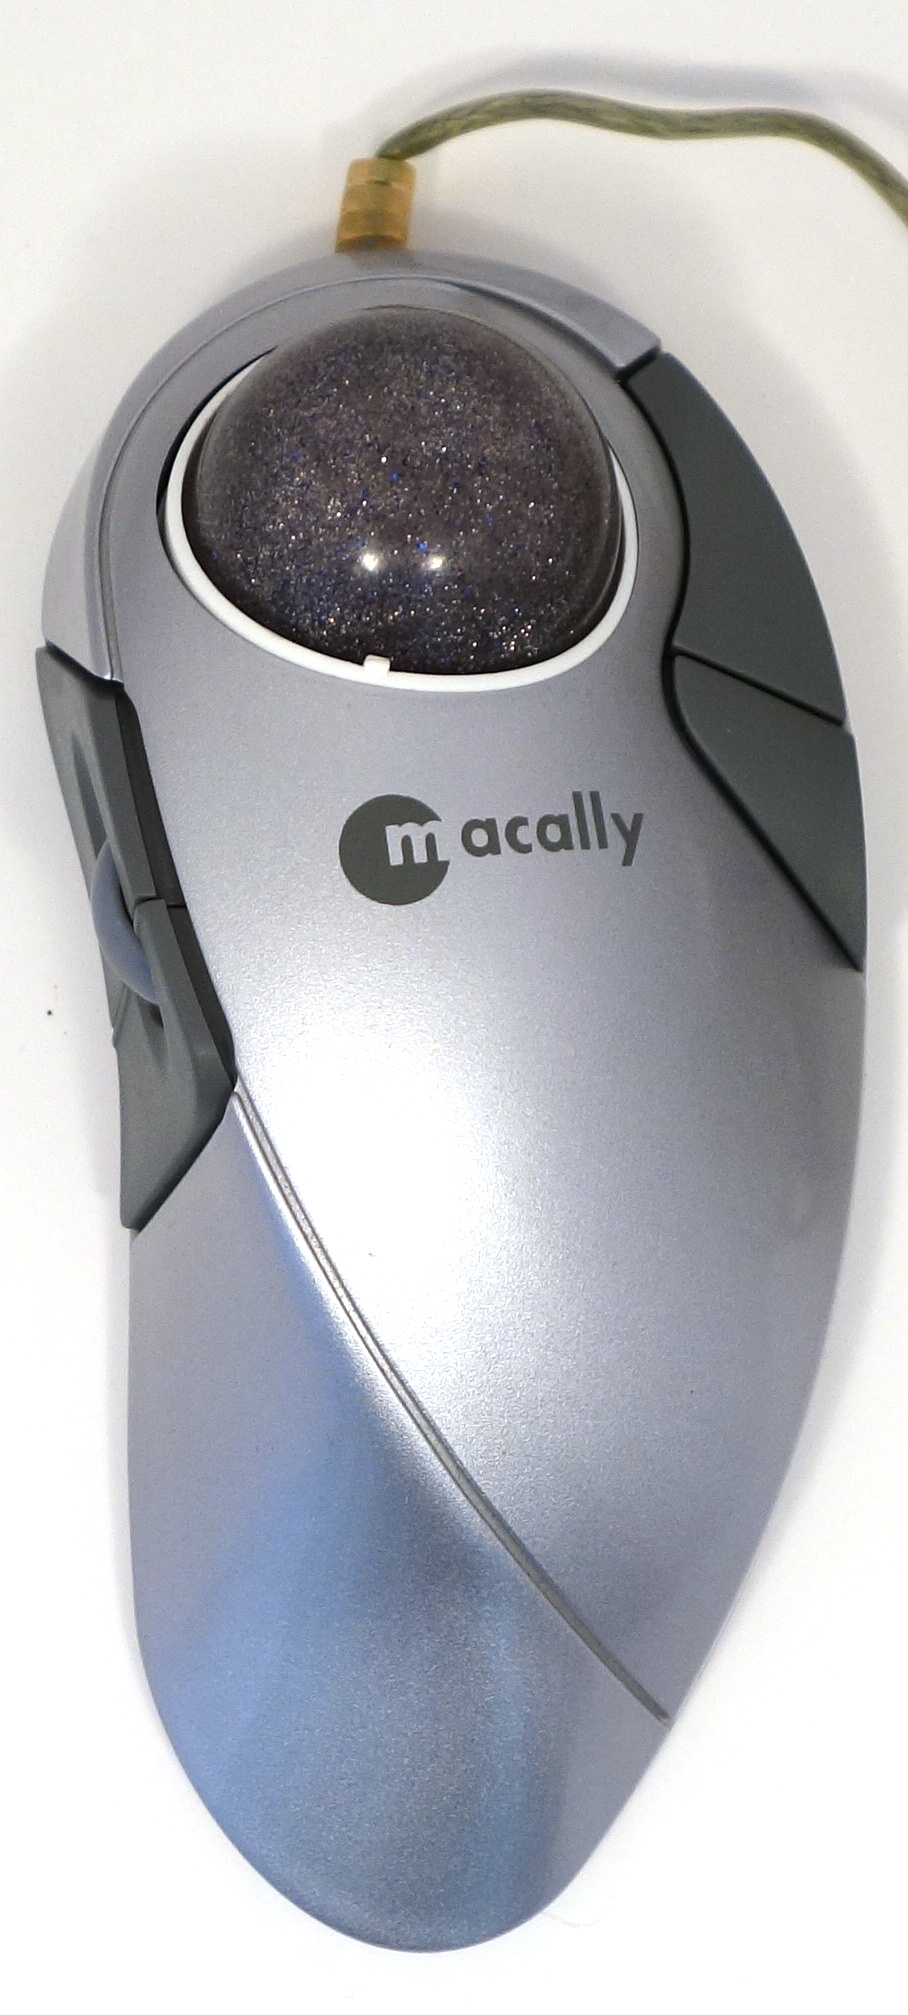
\includegraphics[scale=0.45]{2001_macally_qball/top_30.jpg}
    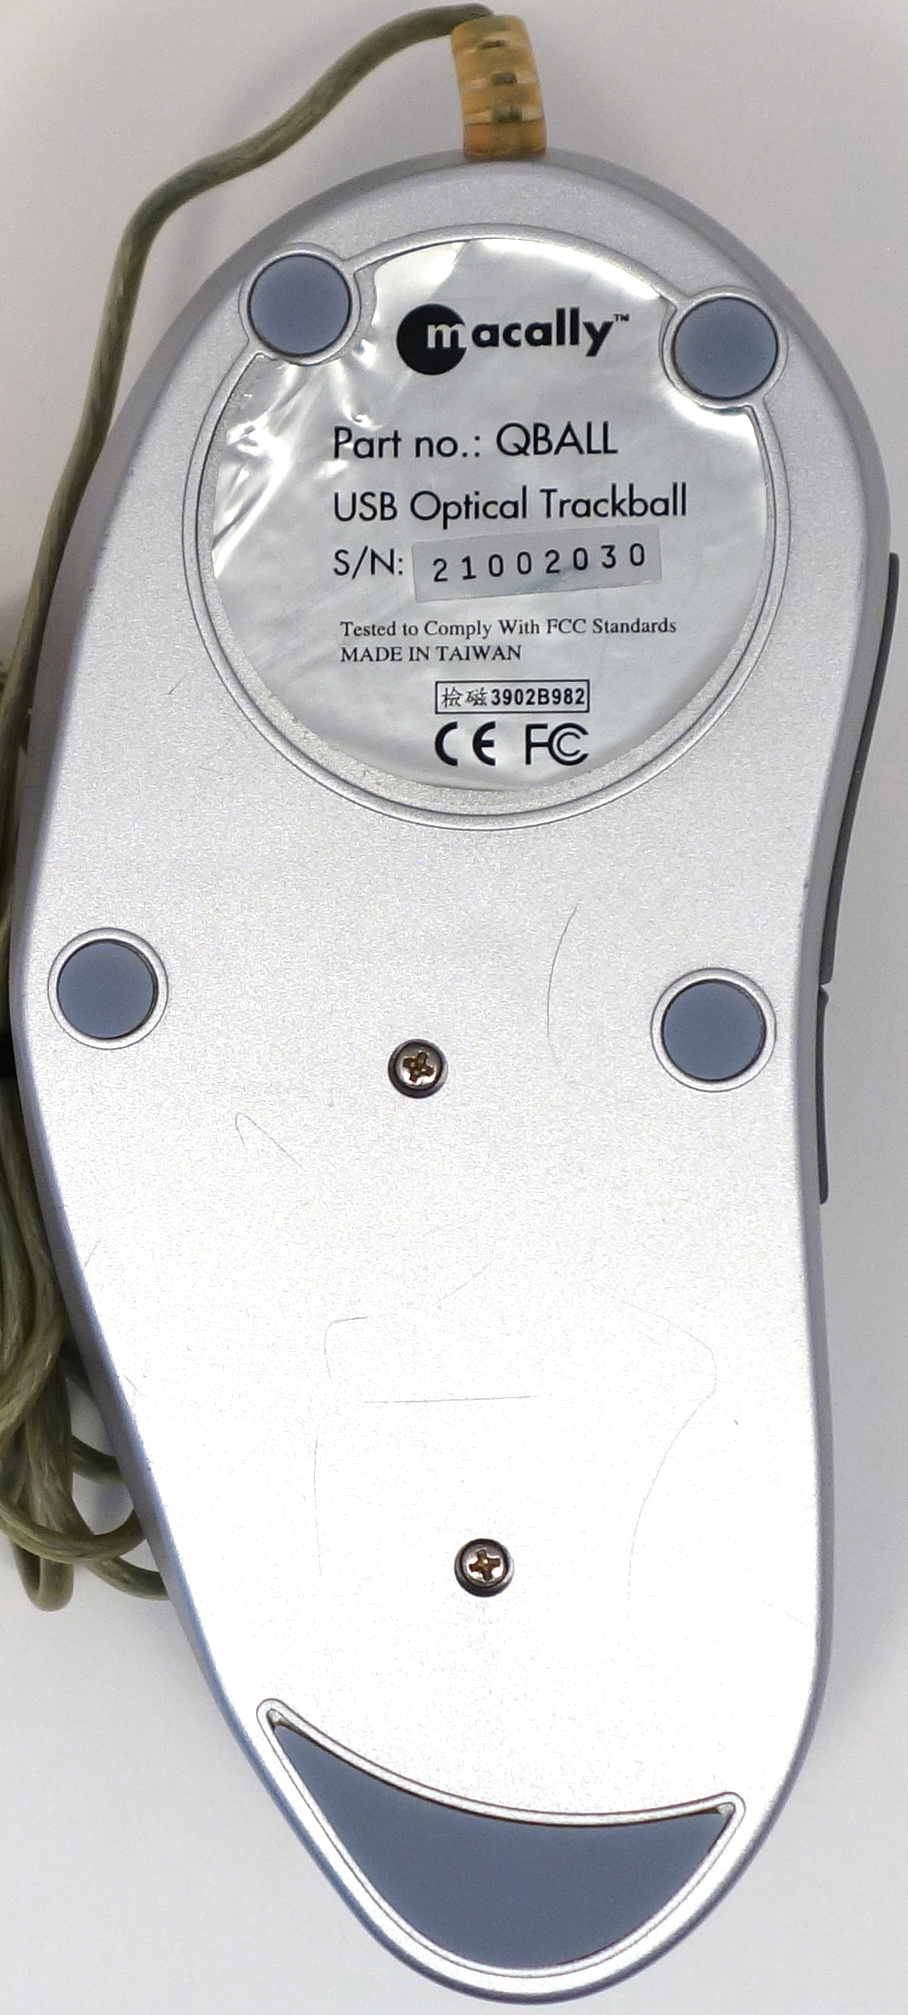
\includegraphics[scale=0.45]{2001_macally_qball/bottom_30.jpg}
    \caption{Macally QBALL, вид сверху и снизу}
    \label{fig:MacallyQBALLTopBottom}
\end{figure}

Этот трекбол имеет асимметричный дизайн (рис. \ref{fig:MacallyQBALLTopBottom}), оснащен 5 кнопками и колесом прокрутки.
Большие левая и правая кнопки возле шара "--- это 1-я и 2-я кнопки мыши, а пара кнопок, расположенных дальше от шара, играет роль 4-й и 5-й.
Кнопка на левой стороне корпуса нажимается большим пальцем вправо, а кнопка на правой стороне нажимается безымянным пальцем. Кнопка, совмещенная с колесом прокрутки, исполняющая традиционную роль 3-й кнопки мыши, нажимается достаточно тяжело, что исключает случайные нажатия при прокрутке.

\begin{figure}[h]
    \centering
    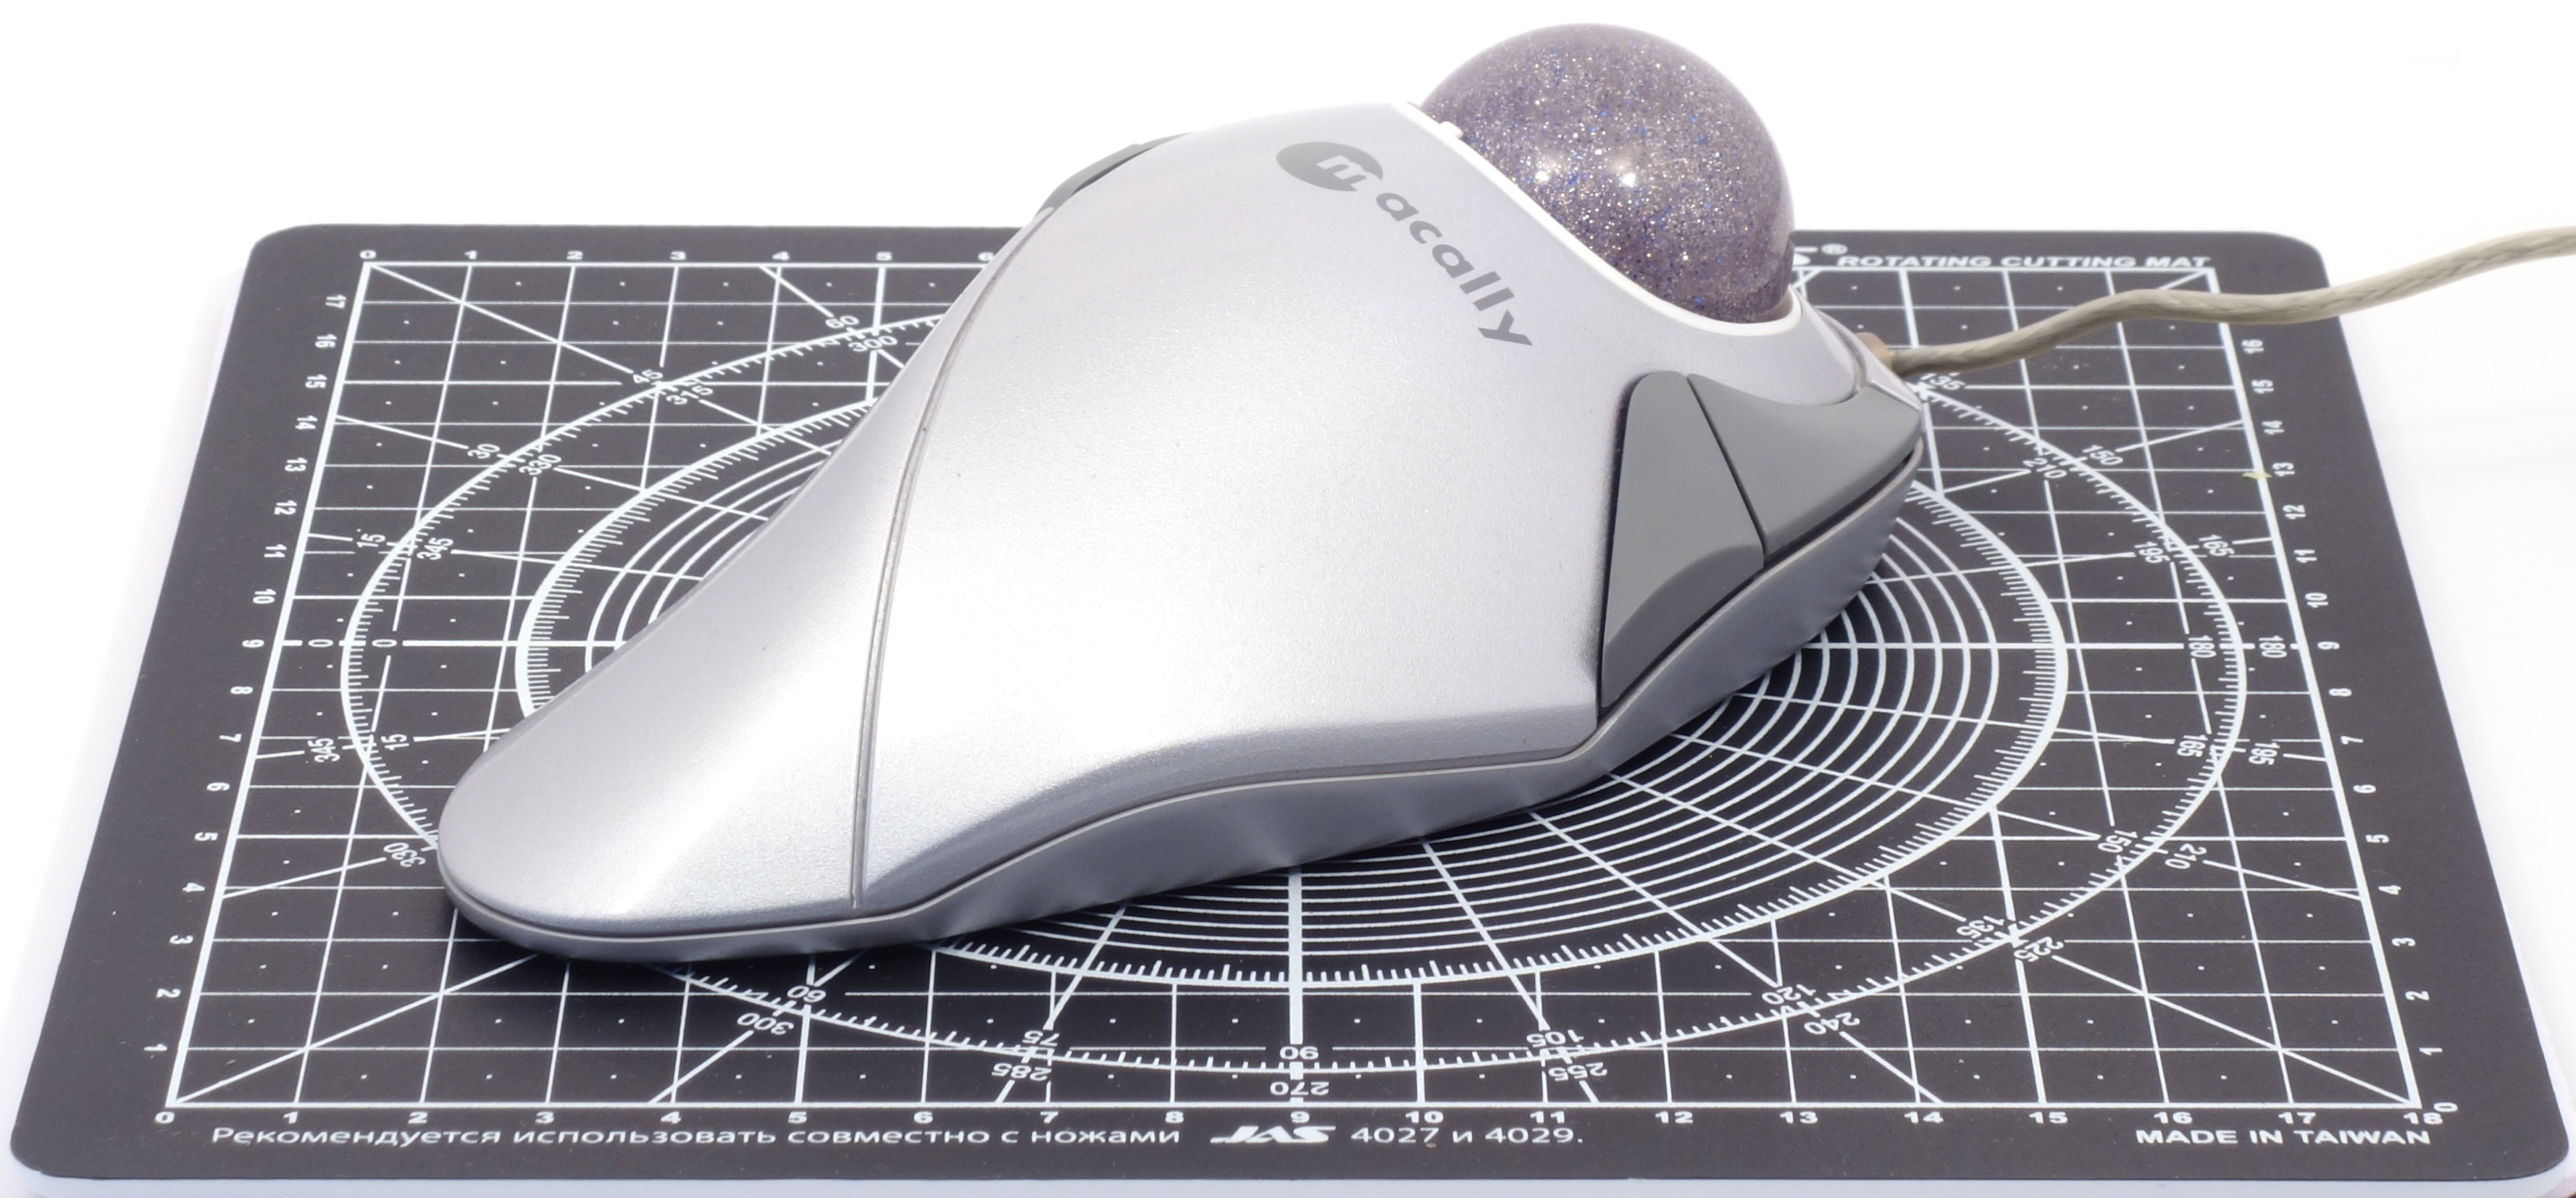
\includegraphics[scale=0.5]{2001_macally_qball/size_30.jpg}
    \caption{Macally QBALL на размерном коврике с шагом сетки 1~см}
    \label{fig:MacallyQBALLSize}
\end{figure}

Создатели QBALL несомненно вдохновлялись моделью Microsoft Trackball Explorer. Можно отметить небольшие различия в форме подставки под запястья и в размерах: QBALL слегка меньше трекбола Microsoft (рис. \ref{fig:MacallyQBALLSize}), но в целом сходство очевидно с первого взгляда.


\begin{figure}[h]
    \centering
    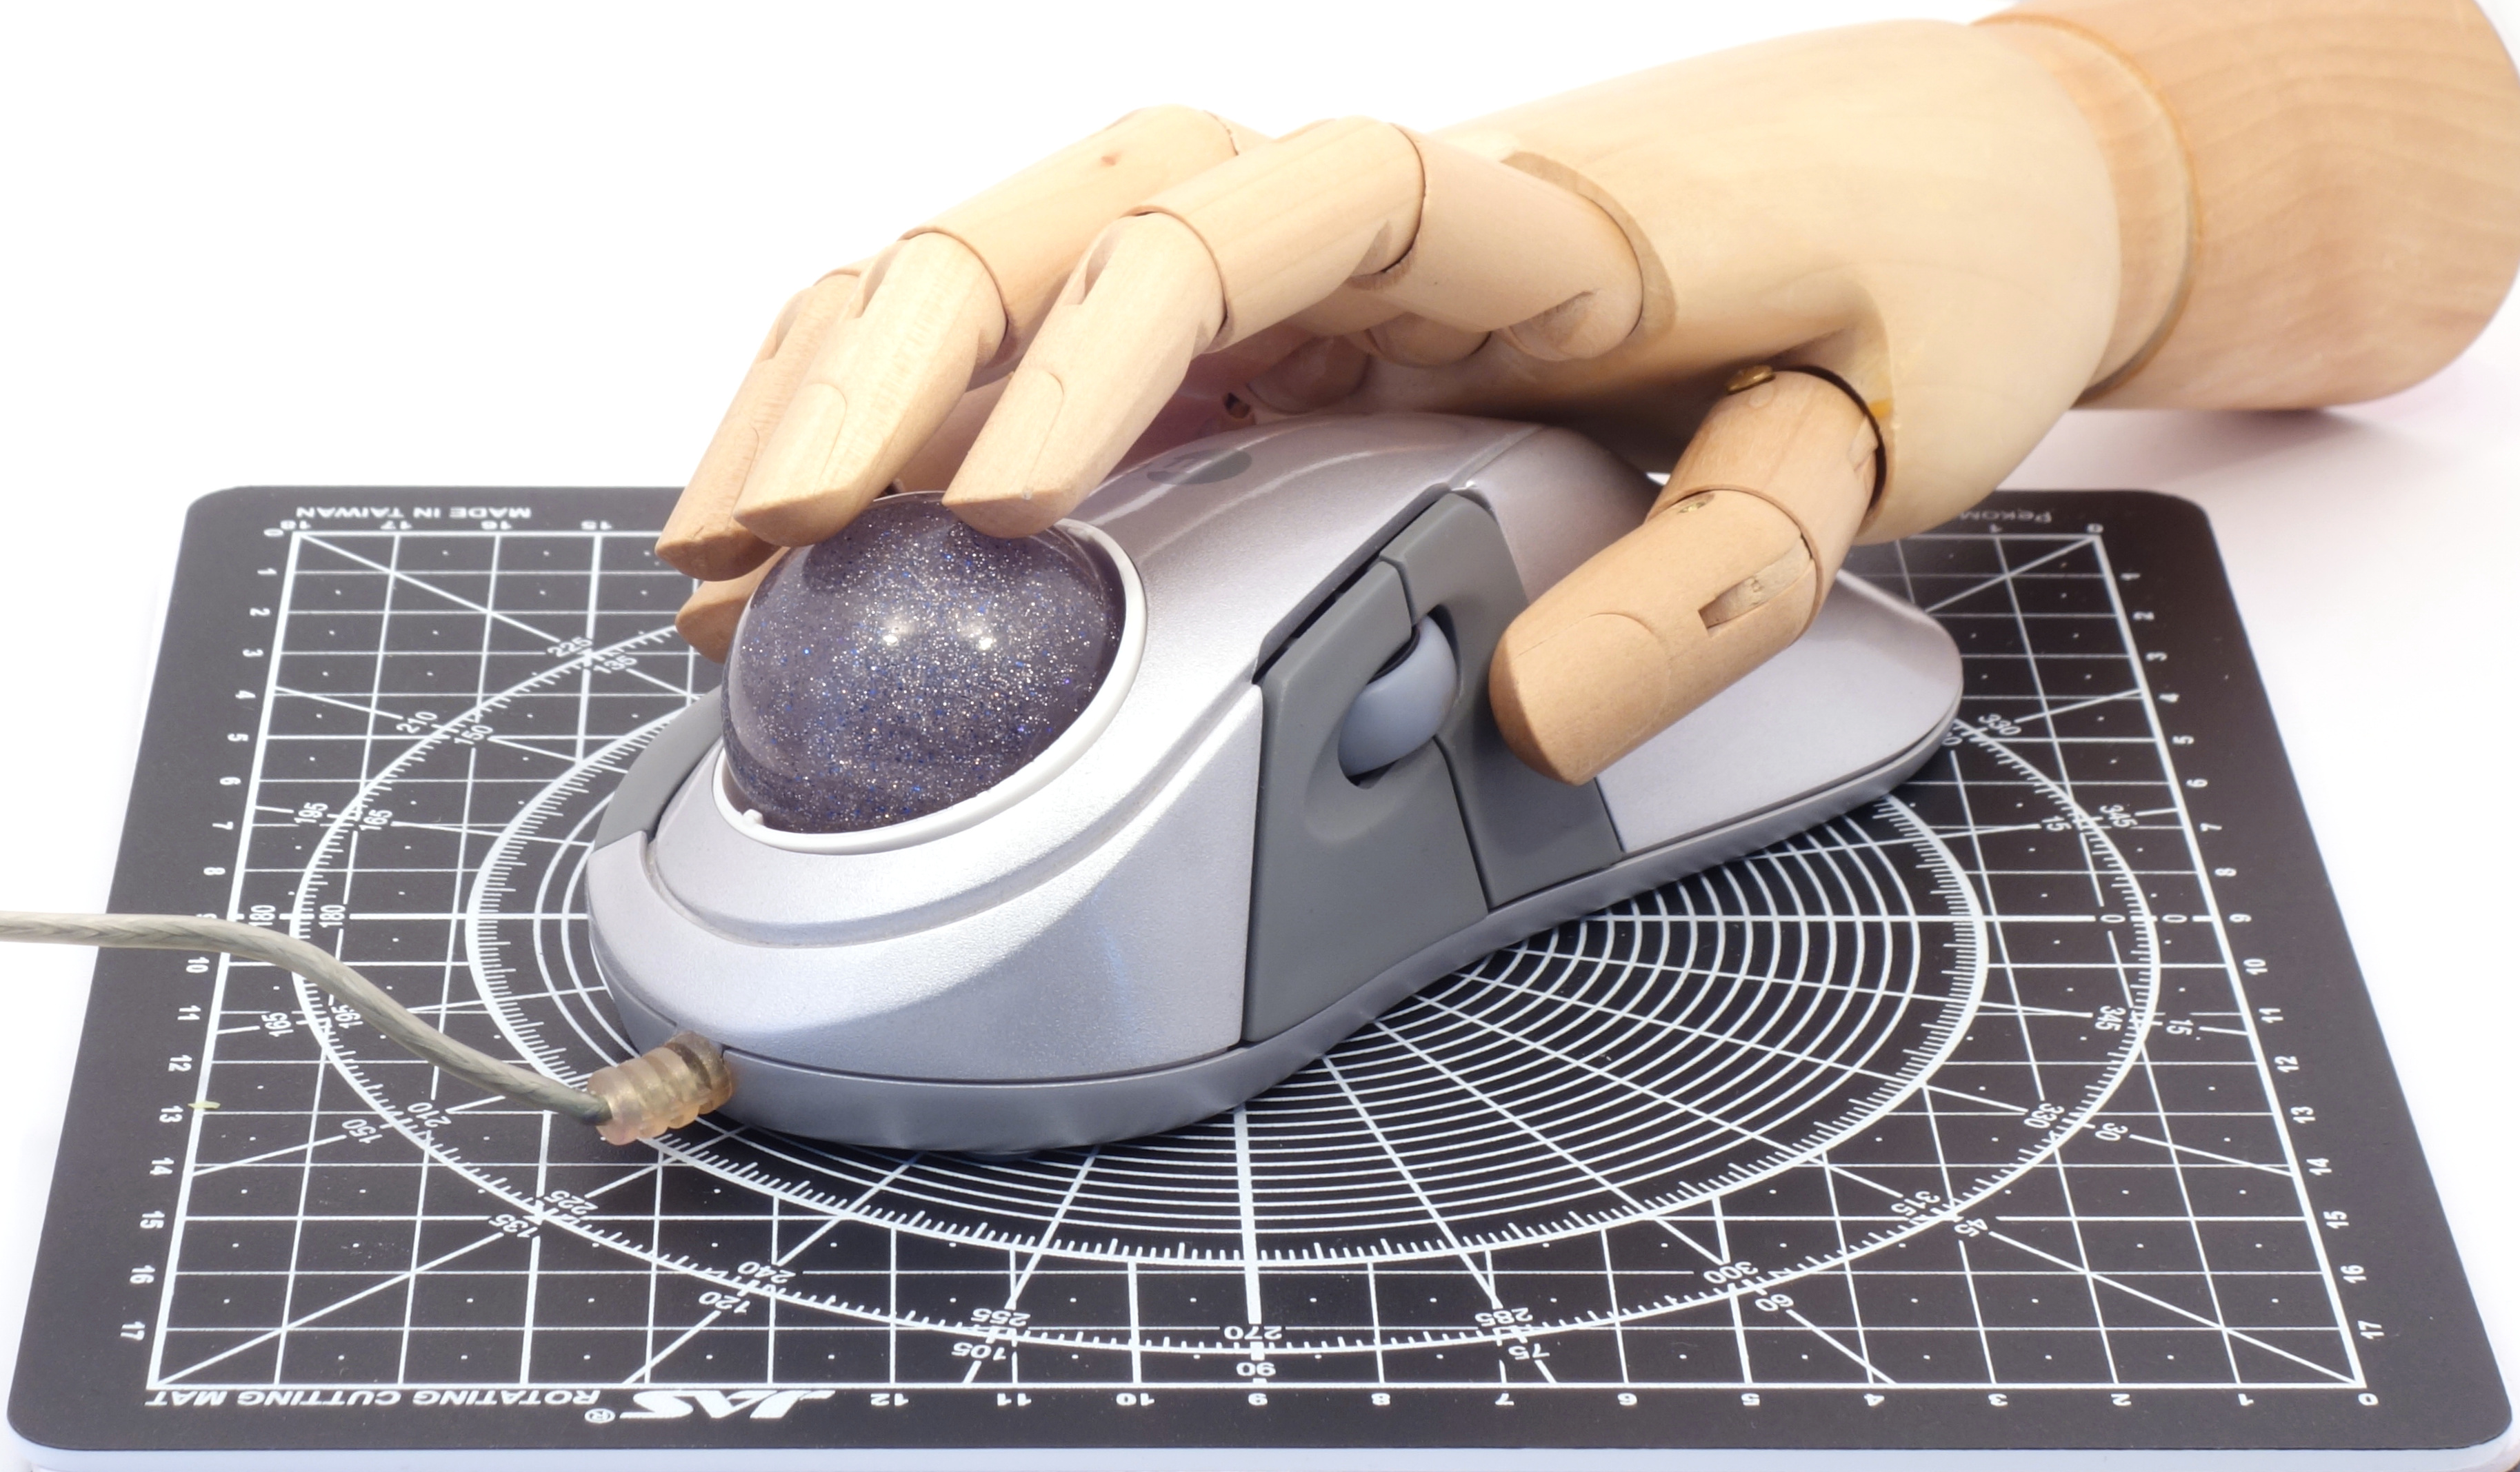
\includegraphics[scale=0.5]{2001_macally_qball/hand_30.jpg}
    \caption{Macally QBALL с моделью руки человека}
    \label{fig:MacallyQBALLHand}
\end{figure}

В плане эргономики можно отметить удобную форму корпуса и удачно расположенные кнопки большого размера (рис. \ref{fig:MacallyQBALLHand}). Асимметричная форма позволяет создать комфортную опору для кисти и удобно расположенное колесо прокрутки, однако делает трекбол подходящим только для правшей.

\begin{figure}[h]
    \centering
    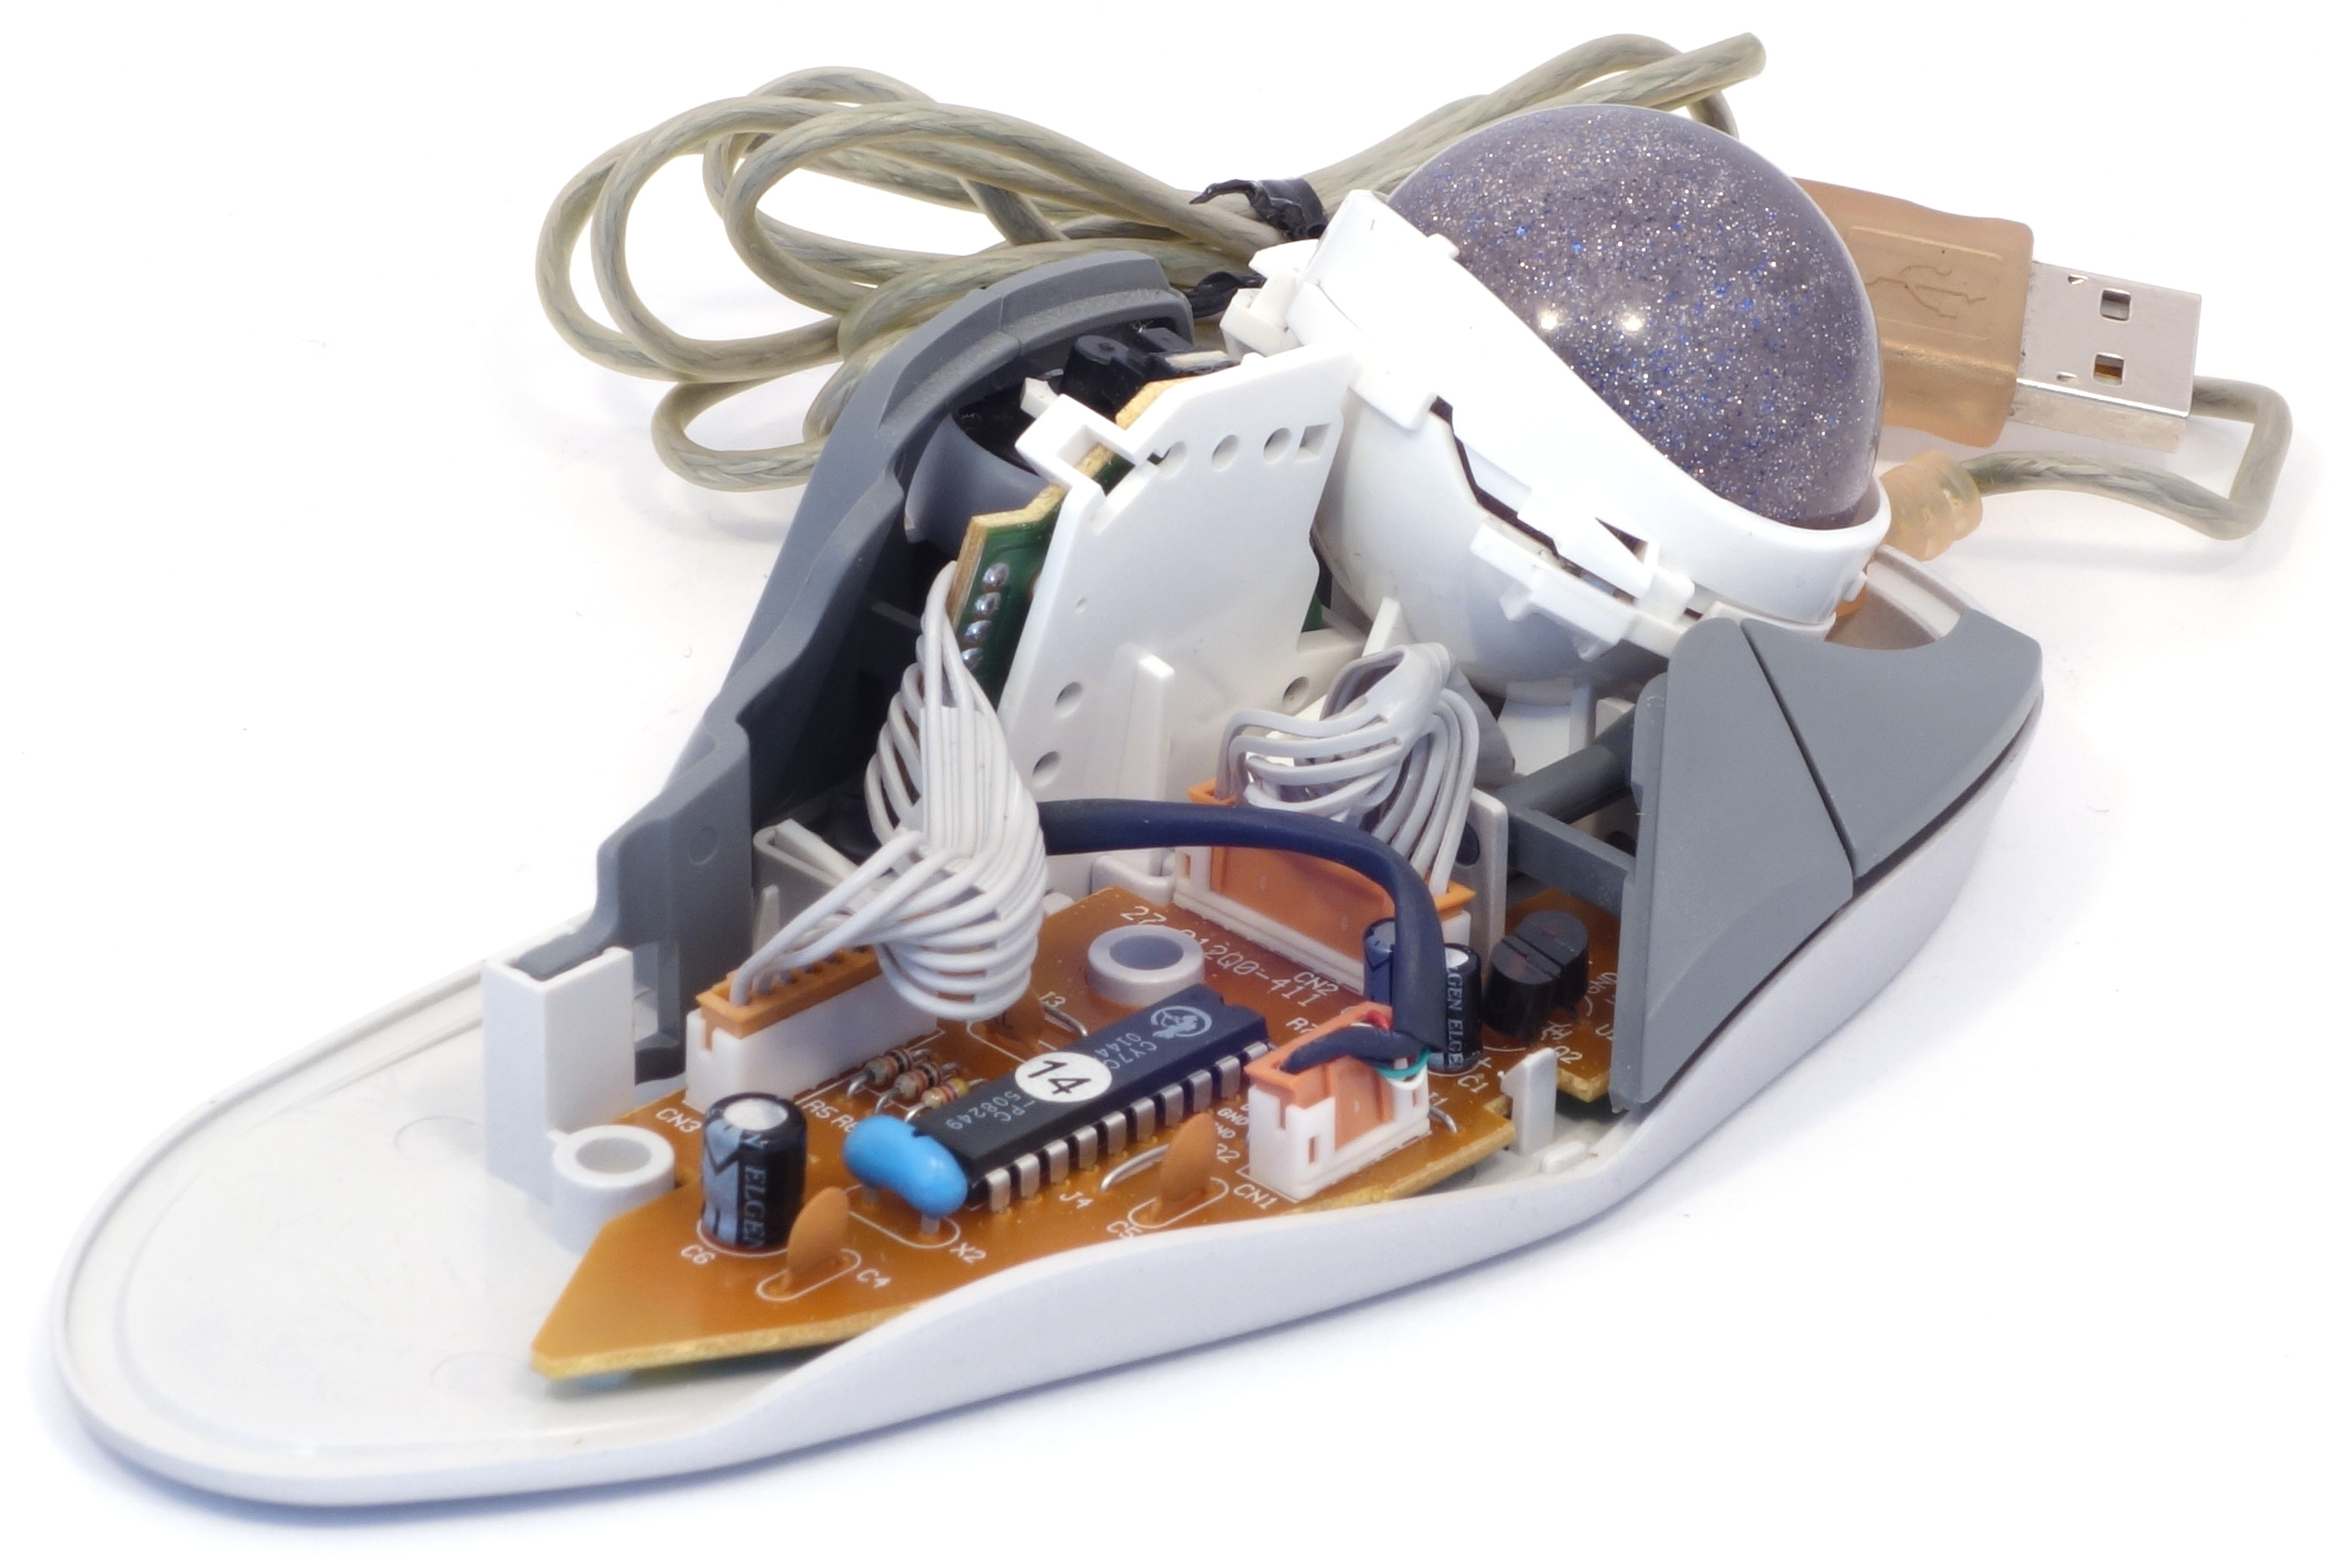
\includegraphics[scale=0.7]{2001_macally_qball/inside_60.jpg}
    \caption{Macally QBALL в разобранном виде}
    \label{fig:MacallyQBALLInside}
\end{figure}

Внутреннее устройство данного трекбола показано на рис. \ref{fig:MacallyQBALLInside}. Как можно видеть, QBALL является полностью оптическим трекболом. Однако, шар опирается на металлические ролики, что типично скорее для оптомеханических трекболов (в большинстве случаев оптических трекболов шар скользит по неподвижным точечным опорам с низким коэффициентом трения).

В \cite{trackballfan} высказывается предположение, что подшипник качения мог быть использован из-за недостаточно гладкой поверхности шара. На официальном ресурсе производителя \cite{site} наличие металлических опорных роликов указывается как дополнительное достоинство модели, обеспечивающее более плавное перемещение шара и меньшую необходимость в регулярной чистке.

\begin{thebibliography}{9}
\bibitem{site} Products -- USB Optical Trackball for Mac \url{https://web.archive.org/web/20010802210604/http://www.macally.com:80/spec/usb/input_device/qball.html}
\bibitem{trackballfan} Trackball Fan! [in Japanese] \url{http://www.hykw.com/tbfan/reviews/pcgb.shtml}
\bibitem{review} VHJ: Review of the Macally Qball in a WinXP Environment \url{https://vanshardware.com/reviews/2004/07/040712_MacallyQball/040712_MacallyQball.htm}
\end{thebibliography}
\end{document}
